
%%%%%%%%%%%%%%%%%%%%%%%%%%%%%%%%%%%%%%%%%%%%%%%%%%%%%%%%%%%%
%%  This Beamer template was created by Cameron Bracken.
%%  Anyone can freely use or modify it for any purpose
%%  without attribution.
%%
%%  Last Modified: January 9, 2009
%%

\documentclass[xcolor={x11names,table},compress,svgnames,mathserif]{beamer}

%% General document %%%%%%%%%%%%%%%%%%%%%%%%%%%%%%%%%%
\usepackage{graphicx}
\usepackage{tikz}
\usepackage{spot}
\usetikzlibrary{mindmap}
\usetikzlibrary{decorations.fractals}
%\usepackage{lmodern}
\usepackage{animate}
\usepackage{movie15}
\usepackage{bm}
\usepackage{pifont}
\usepackage{smartdiagram}
\usepackage[customcolors]{hf-tikz}
\usepackage{empheq}
\usepackage[many]{tcolorbox}
\definecolor{pigment}{rgb}{0.2, 0.2, 0.6}
\definecolor{armygreen}{rgb}{0.29, 0.33, 0.13}
\usepackage{smartdiagram}
\usepackage{booktabs} % for table bottomrule and toprule
\usepackage{changepage} % shift tikzpicture horizontally

\usepackage[absolute,overlay]{textpos}
\DeclareMathOperator*{\argmin}{arg\,min}

% boxed equaton
\usepackage[many]{tcolorbox}

\pgfdeclarehorizontalshading{section shading}{2cm}{
color(0cm)=(LightSlateGrey);
color(2cm)=(gray!7);
color(3cm)=(LightSlateGrey!15)
}

% Custom block environment
% Custom block environment
\newenvironment<>{varblock}[2][.9\textwidth]{%
  \setlength{\textwidth}{#1}
  \begin{actionenv}#3%
    \def\insertblocktitle{#2}%
    \par%
    \usebeamertemplate{block begin}}
  {\par%
    \usebeamertemplate{block end}%
  \end{actionenv}}
  
  %% Algorithm %%%%%
\usepackage[linesnumbered]{algorithm2e}
\newcommand{\nosemic}{\renewcommand{\@endalgocfline}{\relax}}% Drop semi-colon ;
\newcommand{\dosemic}{\renewcommand{\@endalgocfline}{\algocf@endline}}% Reinstate semi-colon ;
\newcommand{\pushline}{\Indp}% Indent
\newcommand{\popline}{\Indm\dosemic}% Undent
\let\oldnl\nl% Store \nl in \oldnl
\newcommand{\nonl}{\renewcommand{\nl}{\let\nl\oldnl}}% Remove line number for one
\SetKwRepeat{Do}{do}{while}
%%%%%%%%%%%%%%%%%

% Vertical line between columns
\newcommand{\vdashrule}[1]{\tikz[remember picture]\draw[dashed,thick,overlay](current page.north)--+(0,-#1);}


%%%%%%%%%%%%%%%%%%%%%%%%%%%%%%%%%%%%%%%%%%%%%%%%%%%%%%

\usetikzlibrary{shapes,arrows,arrows.meta}
\usetikzlibrary{positioning,decorations.pathreplacing}
\tikzstyle{arrow} = [->,>=stealth, line width=1.2pt]
% Define block styles
\tikzstyle{decision} = [diamond, draw, fill=purple!20, 
    text width=5.0em, text badly centered, node distance=3cm, inner sep=0pt]
\tikzstyle{block} = [rectangle, draw=none, fill=blue!20, anchor=north, 
    text width=9.0em, text centered]
    \tikzstyle{blockr} = [rectangle, draw, fill=blue!20, 
    text width=9.0em, text centered, rounded corners]
\tikzstyle{line} = [draw, -latex']
\tikzstyle{cloud} = [draw=none, ellipse,fill=purple!20, node distance=3cm,
    minimum height=2em]
\tikzstyle{startstop} = [rectangle, draw, fill=DeepSkyBlue4,text=white,
   text width=4.5em, text centered, rounded corners]
 \tikzstyle{process} = [rectangle, draw, fill=DeepSkyBlue4,text=white,
   text width=9.0em, text centered]  
 \tikzstyle{io} = [trapezium, fill=DeepSkyBlue4,text=white, trapezium left angle=70, trapezium right angle=110, minimum width=2cm, text width=9.5em,minimum height=1cm, text centered, draw, inner sep=0pt]
    

%% Beamer Layout %%%%%%%%%%%%%%%%%%%%%%%%%%%%%%%%%%
\useoutertheme[subsection=false,shadow]{miniframes}
\useinnertheme{default}
%\usefonttheme{serif}
\usepackage{palatino}
\usepackage{xcolor}
\usepackage{amsmath,amsfonts,amssymb}

\setbeamerfont{title like}{shape=\scshape}
\setbeamerfont{frametitle}{shape=\scshape}
\setbeamertemplate{itemize items}[triangle] % if you wnat a circle
\setbeamertemplate{itemize subitem}[triangle]
\setbeamertemplate{navigation symbols}{}
%\setbeamertemplate{footline}[frame number]

\setbeamercolor{footlinecolor}{fg=white,bg=DeepSkyBlue4}
\defbeamertemplate*{footline}{infolines theme}
{
  \leavevmode%
  \hbox{%
  \begin{beamercolorbox}[wd=.333333\paperwidth,ht=2.25ex,dp=1ex,center]{footlinecolor}
 % {author in head/foot}%
    \usebeamerfont{author in head/foot}\insertshortauthor
   % \usebeamerfont{author in head/foot}\insertshortauthor~~(\insertshortinstitute)
  \end{beamercolorbox}%
  \begin{beamercolorbox}[wd=.333333\paperwidth,ht=2.25ex,dp=1ex,center]{title in head/foot}%
    \usebeamerfont{title in head/foot}\insertshorttitle
  \end{beamercolorbox}%
  \begin{beamercolorbox}[wd=.333333\paperwidth,ht=2.25ex,dp=1ex,right]{footlinecolor}
  %{date in head/foot}%
   % \usebeamerfont{date in head/foot}\insertshortdate{}\hspace*{2em}
    \usebeamerfont{date in head/foot}{manav.vohra@vanderbilt.edu}\hspace*{2em}
    \insertframenumber{} / \inserttotalframenumber\hspace*{2ex} 
  \end{beamercolorbox}}%
  \vskip0pt%
}
%\setbeamercolor{section in head/foot}{fg=white, bg=DeepSkyBlue4}

\setbeamercolor*{lower separation line head}{bg=DeepSkyBlue4} 
\setbeamercolor*{normal text}{fg=black,bg=white} 
\setbeamercolor*{alerted text}{fg=red} 
\setbeamercolor*{example text}{fg=black} 
\setbeamercolor*{structure}{fg=black} 
 
\setbeamercolor*{palette tertiary}{fg=black,bg=black!10} 
\setbeamercolor*{palette quaternary}{fg=black,bg=black!10} 

\renewcommand{\(}{\begin{columns}}
\renewcommand*\footnoterule{}
\renewcommand{\)}{\end{columns}}
\newcommand{\<}[1]{\begin{column}{#1}}
\renewcommand{\>}{\end{column}}

\newcommand*\subitem{%
  \item[\color{DeepSkyBlue4}\scalebox{0.6}{\ding{228}}]}
  
  \newcommand*\subitemtwo{%
  \item[\color{LightSlateGrey!15}\scalebox{0.6}{\ding{228}}]}

\newcommand*\myitem{%
  \item[\color{DeepSkyBlue4}\scalebox{0.6}{\ding{110}}]}
 
  \newcommand*\myitemtwo{%
  \item[\color{LightSlateGrey!15}\scalebox{0.6}{\ding{110}}]}
  
\newcommand*\Myitem{%
  \item[\color{DeepSkyBlue4}\scalebox{0.9}{\ding{42}}]}
  
\newcommand{\be}{\begin{equation}}
\newcommand{\ee}{\end{equation}}
\newcommand{\bea}{\begin{eqnarray}}
\newcommand{\eea}{\end{eqnarray}}
\newcommand{\p}{\partial}
\def\ol{\overline}
\def\no{\noindent}
\def\Vb{{\cal V}}
\def\Qd{\dot{Q}}
\newcommand{\angstrom}{\textup{\AA}}
%\DeclareMathSymbol{\ast}{\mathbin}{symbols}{"03}
 \newcommand{\argmax}{\operatornamewithlimits{arg\,max}}
 

%---------------------QUOTATION--------------------------
\usepackage{etoolbox}
%\usepackage[svgnames]{xcolor}
\usepackage{framed}

% conditional for xetex or luatex
\newif\ifxetexorluatex
\ifxetex
  \xetexorluatextrue
\else
  \ifluatex
    \xetexorluatextrue
  \else
    \xetexorluatexfalse
  \fi
\fi
%
\ifxetexorluatex%
  \usepackage{fontspec}
  \usepackage{libertine} % or use \setmainfont to choose any font on your system
  \newfontfamily\quotefont[Ligatures=TeX]{Linux Libertine O} % selects Libertine as the quote font
\else
  \usepackage[utf8]{inputenc}
  \usepackage[T1]{fontenc}
  %\usepackage{libertine} % or any other font package
  \newcommand*\quotefont{\fontfamily{LinuxLibertineT-LF}} % selects Libertine as the quote font
\fi

\newcommand*\quotesize{30} % if quote size changes, need a way to make shifts relative
% Make commands for the quotes
\newcommand*{\openquote}
   {\tikz[remember picture,overlay,xshift=-3ex,yshift=-0.5ex]
   \node (OQ) {\quotefont\fontsize{\quotesize}{\quotesize}\selectfont``};\kern0pt}

\newcommand*{\closequote}[1]
  {\tikz[remember picture,overlay,xshift=-15ex,yshift={#1}]
   \node (CQ) {\quotefont\fontsize{\quotesize}{\quotesize}\selectfont''};}

% select a colour for the shading
\colorlet{shadecolor}{Azure}

\newcommand*\shadedauthorformat{\emph} % define format for the author argument

% Now a command to allow left, right and centre alignment of the author
\newcommand*\authoralign[1]{%
  \if#1l
    \def\authorfill{}\def\quotefill{\hfill}
  \else
    \if#1r
      \def\authorfill{\hfill}\def\quotefill{}
    \else
      \if#1c
        \gdef\authorfill{\hfill}\def\quotefill{\hfill}
      \else\typeout{Invalid option}
      \fi
    \fi
  \fi}
% wrap everything in its own environment which takes one argument (author) and one optional argument
% specifying the alignment [l, r or c]
%
\newenvironment{shadequote}[2][l]%
{\authoralign{#1}
\ifblank{#2}
   {\def\shadequoteauthor{}\def\yshift{-2ex}\def\quotefill{\hfill}}
   {\def\shadequoteauthor{\par\authorfill\shadedauthorformat{#2}}\def\yshift{2ex}}
\begin{snugshade}\begin{quote}\openquote}
{\shadequoteauthor\quotefill\closequote{\yshift}\end{quote}\end{snugshade}}


%%%%%%%%%%%%%%%%%%%%%%%%%%%%%%%%%%%%%%%%%%%%%%%%%%

\title[Dimension Reduction: Chemical Kinetics]{\textbf{Efficient UQ for Chemical Kinetics
using Active Subspaces}}
\thispagestyle{empty}
\pgfsetfillopacity{0.9}
\setbeamercolor{title}{bg=DeepSkyBlue4,fg=white}


%\subtitle{SUBTITLE}
\author[M. Vohra et al.]{Manav Vohra$^{\dag}$, Sankaran Mahadevan$^{\dag}$ \\ \vspace{2mm}
\textbf{Collaborators}: Alen Alexanderian$^{\S}$, Hailey Guy$^{\S}$}
\vspace{-1mm}
\institute{$^{\dag}$Vanderbilt University\\ \vspace{1mm}
$^{\S}$North Carolina State University}

\date{\today}

\begin{document}

%___________________________NEW SLIDE______________________________________
{
\setbeamertemplate{headline}{}

\begin{frame}[noframenumbering]

\titlepage
\vspace{-21mm}
\centering

\end{frame}
}


%___________________________NEW SLIDE______________________________________

\section{Active Subspaces}
\subsection{ac}
\begin{frame}{Background $\&$ Motivation} 
\normalsize
\vspace{2mm}
\begin{itemize}
\myitem \textbf{Idea}: {\color{pigment}Discover} and {\color{pigment}Exploit} a {\color{pigment}low-dimensional}
structure in the model. 

\vspace{2mm}
\begin{table}[htbp]
\scriptsize
\renewcommand*{\arraystretch}{1.2}
\begin{center}
\begin{tabular}{ccc}
\toprule
Parameters & Model Runs & Time (1s/run)\\
\bottomrule
1 & 10 & 10 s \\
2 & 10$^2$ & 1.6 min \\
3 & 10$^3$ & 16 min \\
4 & 10$^4$ & 2.7 hours \\
5 & 10$^5$ & 1.1 days \\
6 & 10$^6$ & 1.6 weeks \\
\bottomrule
\end{tabular}
\end{center}
\end{table}

\tikz[overlay, remember picture] \node at (2.95,3.7) {\tiny{Active Subspaces}};
\tikz[overlay, remember picture] \node at (2.85,1.8) {
\begin{tcolorbox}[width=0.16\textwidth,height=0.32\textwidth,colback=DeepSkyBlue!10,notitle,colframe=DeepSkyBlue!20,colupper=DeepSkyBlue4,enhanced,opacityfill=0.3]
\end{tcolorbox}
};

\myitem \textbf{Definition}: Dominant eigenspace of a matrix derived from the model's gradient. 
\vspace{-4mm}

\begin{center}
%\scriptsize{
\be
\begin{aligned}
\int \nabla f(\bm(x))\nabla f(\bm{x})^\top\rho(\bm{x})d\bm{x} &= W\Lambda W^\top \\ 
\vspace{-2mm}
f(\bm{x}) &= g(w_1^\top x)~~~\text{\tiny{[P. Constantine, 2015]}}
\end{aligned} \nonumber
\ee
 \end{center}

\end{itemize}
\end{frame}

%___________________________NEW SLIDE______________________________________

\section{\scshape Methodology}
\subsection{ac}
\begin{frame}{Gradient-based Approach} 

\end{frame}


%___________________________NEW SLIDE______________________________________

\subsection{ac}
\begin{frame}{Adaptive Gradient-free Approach} 

\end{frame}

%___________________________NEW SLIDE______________________________________

\section{\scshape Application}
\subsection{ac}
\begin{frame}{H$_2$/O$_2$ Reaction Kinetics}
\normalsize
\begin{columns}
\begin{column}{0.55\textwidth}
\begin{itemize}
\myitem Reaction Rate:
\vspace{2mm}
\begin{tcolorbox}[width=0.65\textwidth,height=0.15\textwidth,colback=DeepSkyBlue!10,notitle,colframe=DeepSkyBlue!20,colupper=DeepSkyBlue4]
\vspace{-5.5mm}
\scriptsize
\be
\hspace{-4.2mm}
k_i(T) = A_iT^{n_i}\exp(-E_{a,i}/RT) \nonumber
\ee
\end{tcolorbox}
\tiny \vspace{-1mm}
$A_i$: Pre-exponent~~~$E_{a,i}$: Activation Energy
\normalsize \vspace{1mm}
\myitem Uniform Priors:  \scriptsize $A_i\in[0.9A_i^\ast, 1.1A_i^\ast]$, $E_{a,i}\in[0.9E_{a,i}^\ast, 1.1E_{a,i}^\ast]$
\vspace{1mm}
\normalsize

\myitem Global Reaction:
\vspace{2mm}
\begin{tcolorbox}[width=0.42\textwidth,height=0.15\textwidth,colback=DeepSkyBlue!10,notitle,colframe=DeepSkyBlue!20,colupper=DeepSkyBlue4]
\vspace{-5.5mm}
\scriptsize
\be
\hspace{-4.2mm}
2\text{H}_2 + \text{O}_2 \rightarrow 2\text{H}_2\text{O} \nonumber
\ee
\end{tcolorbox}

\vspace{-1mm}
\normalsize

\myitem Equivalence Ratio ($\phi$):
\vspace{1mm}
\begin{tcolorbox}[width=0.45\textwidth,height=0.2\textwidth,colback=DeepSkyBlue!10,notitle,colframe=DeepSkyBlue!20,colupper=DeepSkyBlue4]
\vspace{-5.5mm}
\scriptsize
\be
\hspace{-4.2mm}
\phi = \frac{(M_{\text{H}_2}/M_{\text{O}_2})_\text{obs}}{(M_{\text{H}_2}/M_{\text{O}_2})_\text{st}}~~~~
\tiny{{\color{black}\phi > 1: \text{Rich},~\phi < 1: \text{Lean}}}
 \nonumber
\ee
\end{tcolorbox}

\end{itemize}
\end{column}
\hspace{3mm}
\begin{column}{0.45\textwidth}
\vspace{-5mm}
\begin{table}[htbp]
\renewcommand*{\arraystretch}{1.2}
\begin{center}
\resizebox{\columnwidth}{!}{%
\begin{tabular}{llll}
\toprule
Reaction \#     & Reactants & & Products\\
\bottomrule
$\mathcal{R}_1$ & H + O$_2$          & $\rightleftharpoons$ & O + OH \\
$\mathcal{R}_2$ & O + H$_2$          & $\rightleftharpoons$ & H + OH \\
$\mathcal{R}_3$ & H$_2$ + OH         & $\rightleftharpoons$ & H$_2$O + H \\
$\mathcal{R}_4$ & OH + OH            & $\rightleftharpoons$ & O + H$_2$O \\
$\mathcal{R}_5$ & H$_2$ + M          & $\rightleftharpoons$ & H + H + M \\
$\mathcal{R}_6$ & O + O + M          & $\rightleftharpoons$ & O$_2$ + M \\
$\mathcal{R}_7$ & O + H + M          & $\rightleftharpoons$ & OH + M \\
$\mathcal{R}_8$ & H + OH +M          & $\rightleftharpoons$ & H$_2$O + M \\
$\mathcal{R}_9$ & H + O$_2$ + M      & $\rightleftharpoons$ & HO$_2$ + M \\
$\mathcal{R}_{10}$ & HO$_2$ + H      & $\rightleftharpoons$ & H$_2$ + O$_2$ \\
$\mathcal{R}_{11}$ & HO$_2$ + H      & $\rightleftharpoons$ & OH + OH \\
$\mathcal{R}_{12}$ & HO$_2$ + O      & $\rightleftharpoons$ & O$_2$ + OH \\
$\mathcal{R}_{13}$ & HO$_2$ + OH     & $\rightleftharpoons$ & H$_2$O + O$_2$ \\
$\mathcal{R}_{14}$ & HO$_2$ + HO$_2$ & $\rightleftharpoons$ & H$_2$O$_2$ + O$_2$ \\
$\mathcal{R}_{15}$ & H$_2$O$_2$ + M  & $\rightleftharpoons$ & OH + OH + M \\
$\mathcal{R}_{16}$ & H$_2$O$_2$ + H  & $\rightleftharpoons$ & H$_2$O + OH \\
$\mathcal{R}_{17}$ & H$_2$O$_2$ + H  & $\rightleftharpoons$ & HO$_2$ + H$_2$ \\
$\mathcal{R}_{18}$ & H$_2$O$_2$ + O  & $\rightleftharpoons$ & OH + HO$_2$ \\
$\mathcal{R}_{19}$ & H$_2$O$_2$ + OH & $\rightleftharpoons$ & HO$_2$ + H$_2$O \\
\bottomrule
\end{tabular}
}
\\ \vspace{1mm}
\tiny{[Yetter et al., 1991]}
\end{center}
\end{table}

\end{column}
\end{columns}
\end{frame}

%___________________________NEW SLIDE______________________________________

\section{\scshape Results}
\subsection{res}
\begin{frame}{Convergence: Eigenvalues} 
\begin{center}
        \animategraphics[poster=first,controls,height=0.4\textwidth]{5}
       {./Figures/eig_comp}{1}{5}
\end{center}
\end{frame}

%___________________________NEW SLIDE______________________________________

\subsection{res}
\begin{frame}{Convergence: Eigenvectors} 

\begin{columns}
\begin{column}{0.5\textwidth}
 \begin{center}
  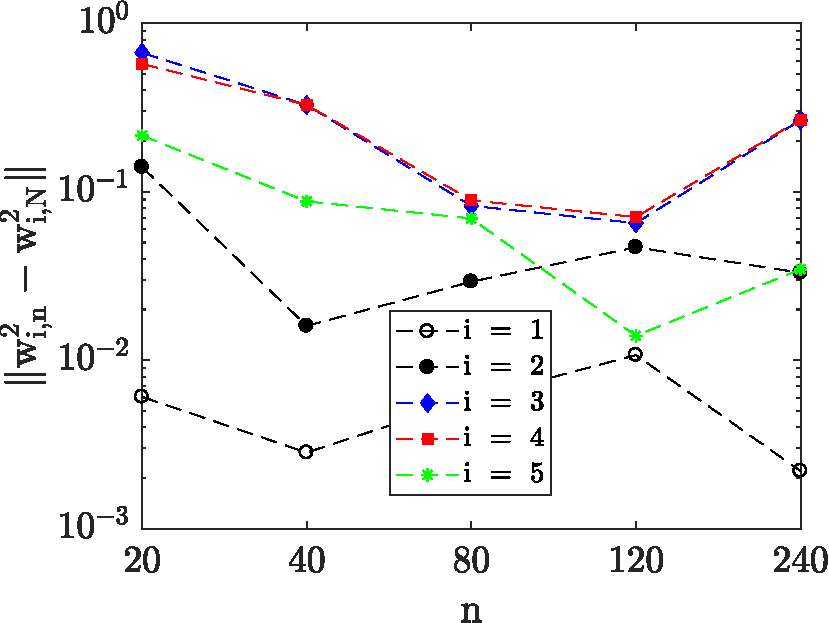
\includegraphics[width=0.88\textwidth]{./Figures/err_eigv_1_5}
   \\ \vspace{2mm}
  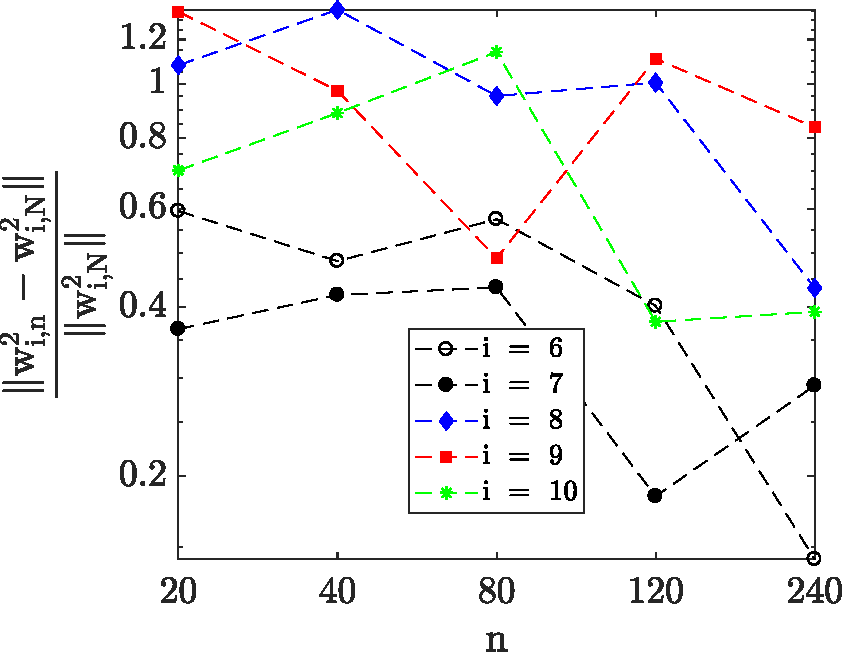
\includegraphics[width=0.85\textwidth]{./Figures/err_eigv_6_10}
\end{center}
\end{column}
%\hspace{-20mm}
\begin{column}{0.5\textwidth}
 \begin{center}
  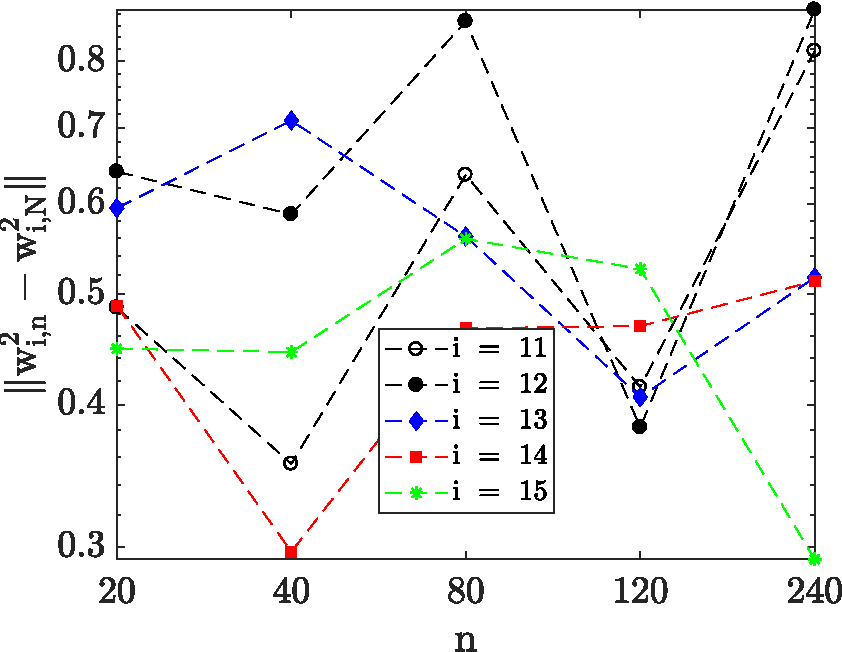
\includegraphics[width=0.8\textwidth]{./Figures/err_eigv_11_15}
   \\ \vspace{2mm}
  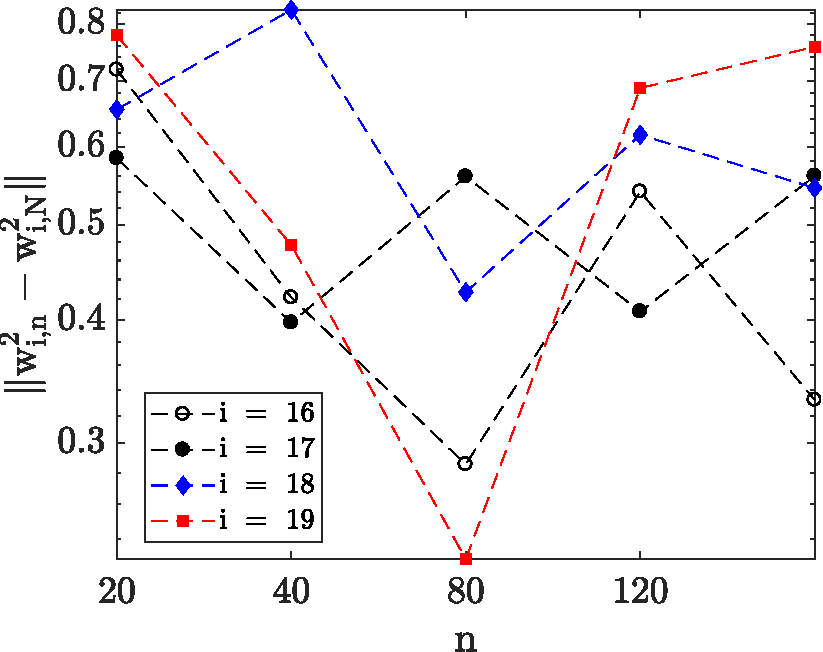
\includegraphics[width=0.82\textwidth]{./Figures/err_eigv_16_19}
\end{center}
\end{column}
\end{columns}

\end{frame}

%___________________________NEW SLIDE______________________________________

\subsection{res}
\begin{frame}{Comparative Assessment} 

\begin{center}
        \animategraphics[poster=first,controls,height=0.4\textwidth]{5}
       {./Figures/eigv}{1}{6}
\end{center}

\end{frame}

%___________________________NEW SLIDE______________________________________

\subsection{res}
\begin{frame}{Comparative Assessment} 

\begin{columns}
\begin{column}{0.5\textwidth}
 \begin{center}
\vspace{1.7mm}
  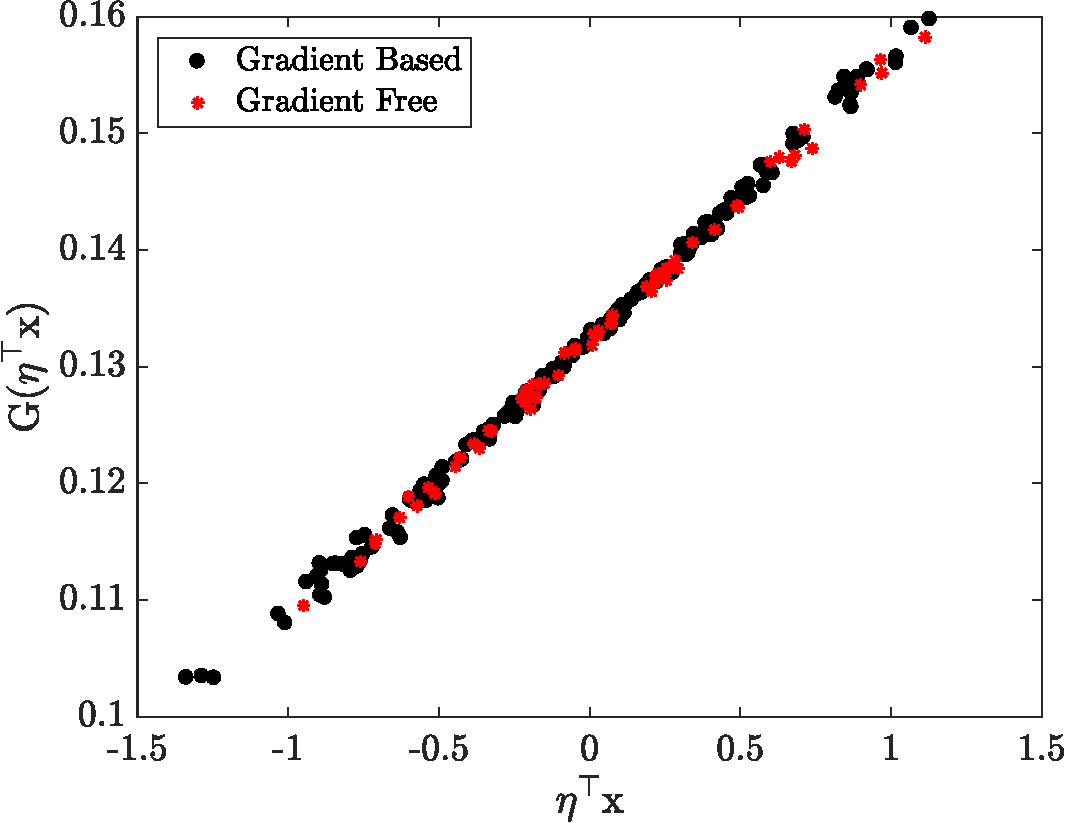
\includegraphics[width=0.95\textwidth]{./Figures/comp_ssp}
\end{center}
\end{column}
%\hspace{-20mm}
\begin{column}{0.5\textwidth}
 \begin{center}
  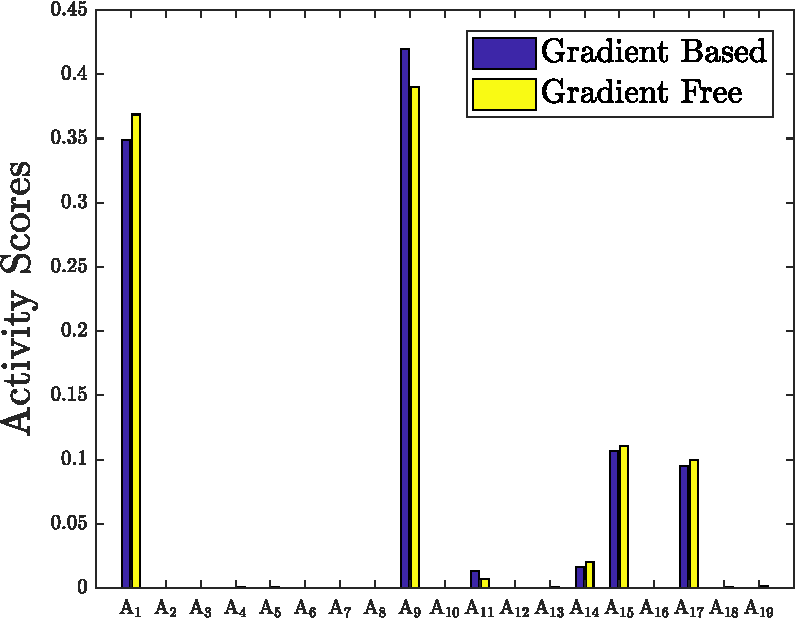
\includegraphics[width=0.85\textwidth]{./Figures/comp_as}
\end{center}
\end{column}
\end{columns}

\end{frame}

%___________________________NEW SLIDE______________________________________

\subsection{res}
\begin{frame}{Sensitivity Analysis} 

\begin{columns}
\begin{column}{0.5\textwidth}
\begin{itemize}
\myitem Sobol total effect index
\scriptsize
\begin{align}
\mathcal{T}(\theta_i) &= 
1 - \frac{\mathbb{V}_{\bm{\theta}_{\sim i}}(\mathbb{E}_{\theta_i}[\mathcal{G}\vert\bm{\theta}_{\sim i}])}{\mathbb{V}(\mathcal{G})} \nonumber \\ \vspace{1mm}
&= \frac{\frac{1}{N}\sum\limits_{k=1}^{N}f(\bm{A})_k(f(\bm{A})_k - f(\bm{A_B}^i)_k)}{\mathbb{V}(\mathcal{G})} \nonumber
\end{align}

\begin{itemize}
\scriptsize
\item $\bm{A}$, $\bm{B}$: Matrices comprising independent samples of $\bm{\theta}$.  \vspace{2mm}
\item $\bm{A_B}^i$: $i^{\text{th}}$ column of A is replaced by the  $i^{\text{th}}$ column of $\bm{B}$.
\end{itemize}

\normalsize
\vspace{3mm}
\myitem Activity scores
\vspace{-2mm}
\scriptsize
\be
\alpha_i(n) = \sum\limits_{j=1}^n \lambda_jv_{i,j}^2 \nonumber
\ee

\end{itemize}
\end{column}

\begin{column}{0.5\textwidth}

\begin{figure}[htbp]
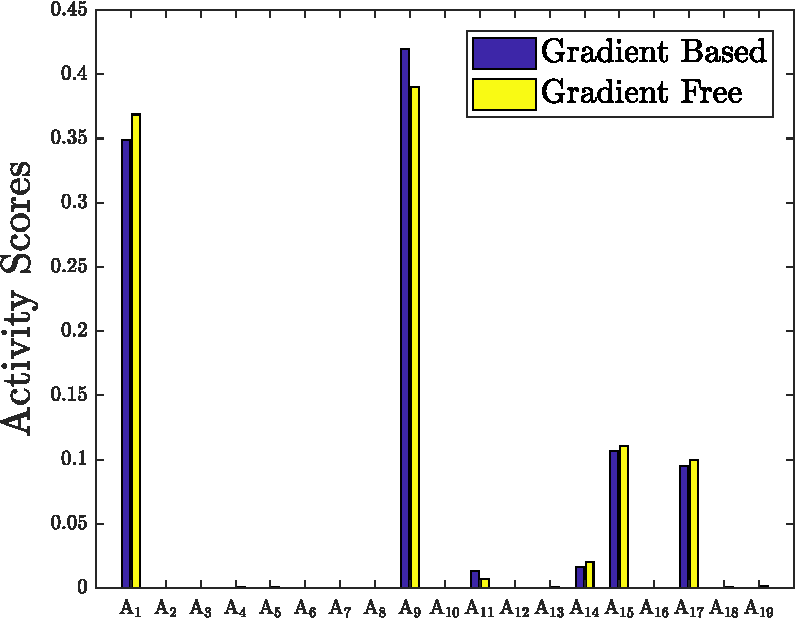
\includegraphics[width=0.8\textwidth]{./Figures/comp_as}
\\ \vspace{5mm}
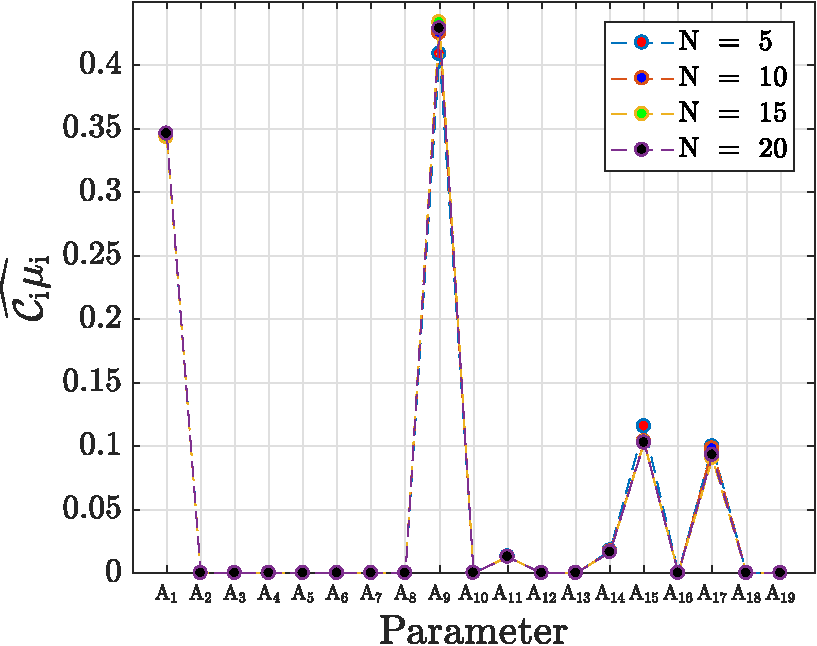
\includegraphics[width=0.8\textwidth]{./Figures/ub_conv_kinetics_rich}
\end{figure}

\end{column}
\end{columns}

\end{frame}

%___________________________NEW SLIDE______________________________________

\subsection{res}
\begin{frame}{High-Dimensional Problem} 

\begin{columns}
\begin{column}{0.5\textwidth}

\begin{center}
\begin{figure}[htbp]
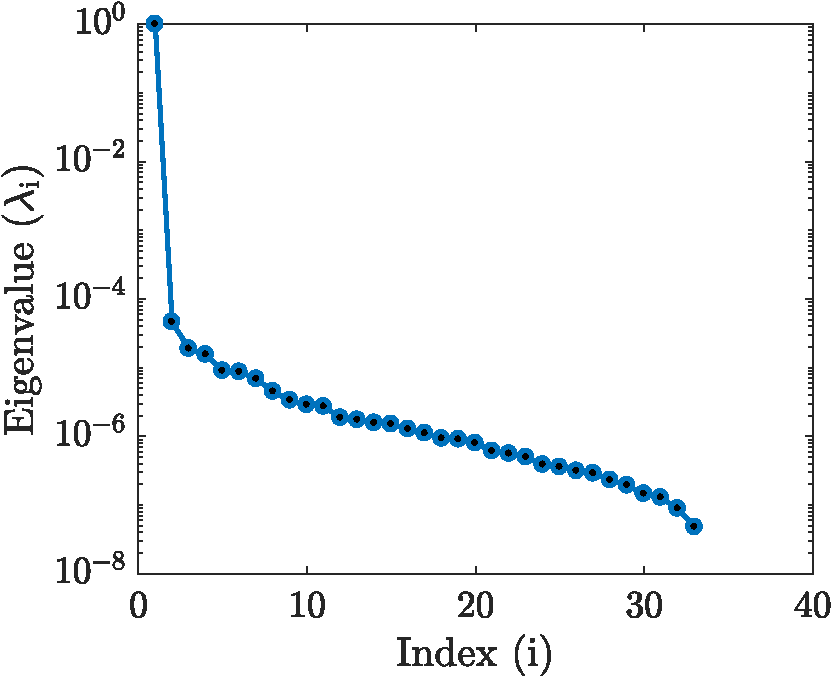
\includegraphics[width=0.78\textwidth]{./Figures/eig_33D}
\end{figure}
\end{center}

\end{column}

\hspace{-15mm}
\begin{column}{0.5\textwidth}

\begin{center}
\begin{figure}[htbp]
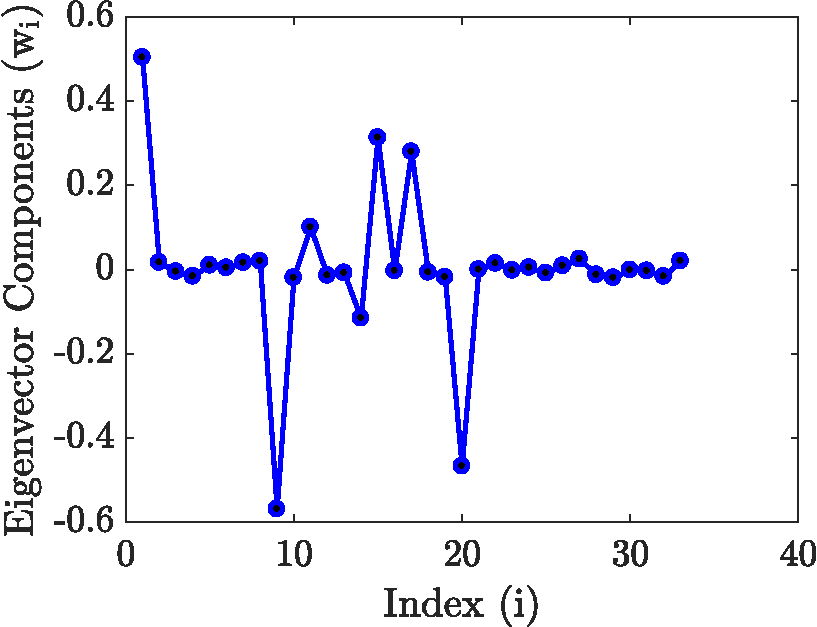
\includegraphics[width=0.78\textwidth]{./Figures/eigv_33D}
\end{figure}
\end{center}

\end{column}
\end{columns}

\begin{center}
\begin{figure}[htbp]
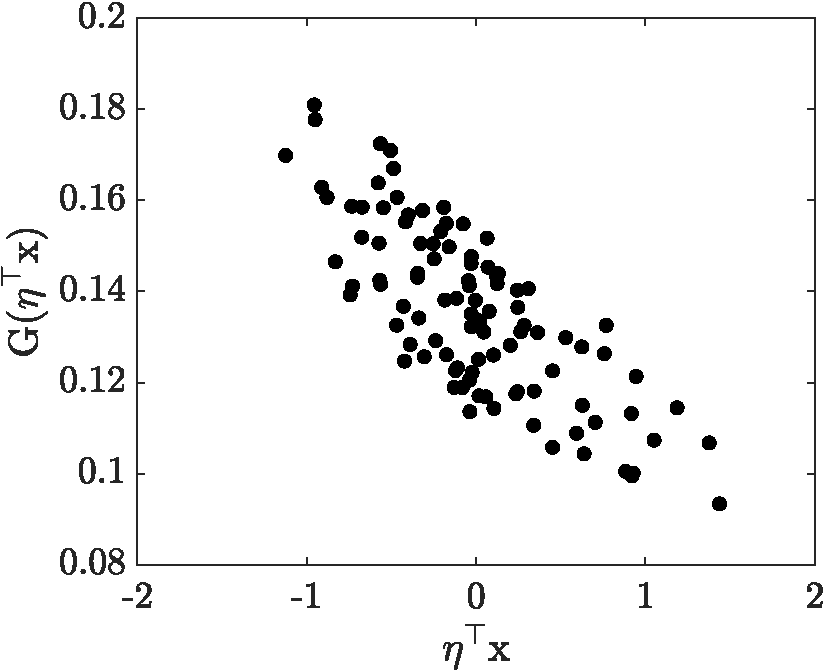
\includegraphics[width=0.40\textwidth]{./Figures/ssp_33D}
\end{figure}
\end{center}

\end{frame}

%___________________________NEW SLIDE______________________________________

\subsection{res}
\begin{frame}{Sensitivity Analysis} 

\vspace{-3mm}
\begin{figure}[htbp]
\hspace{-5mm}
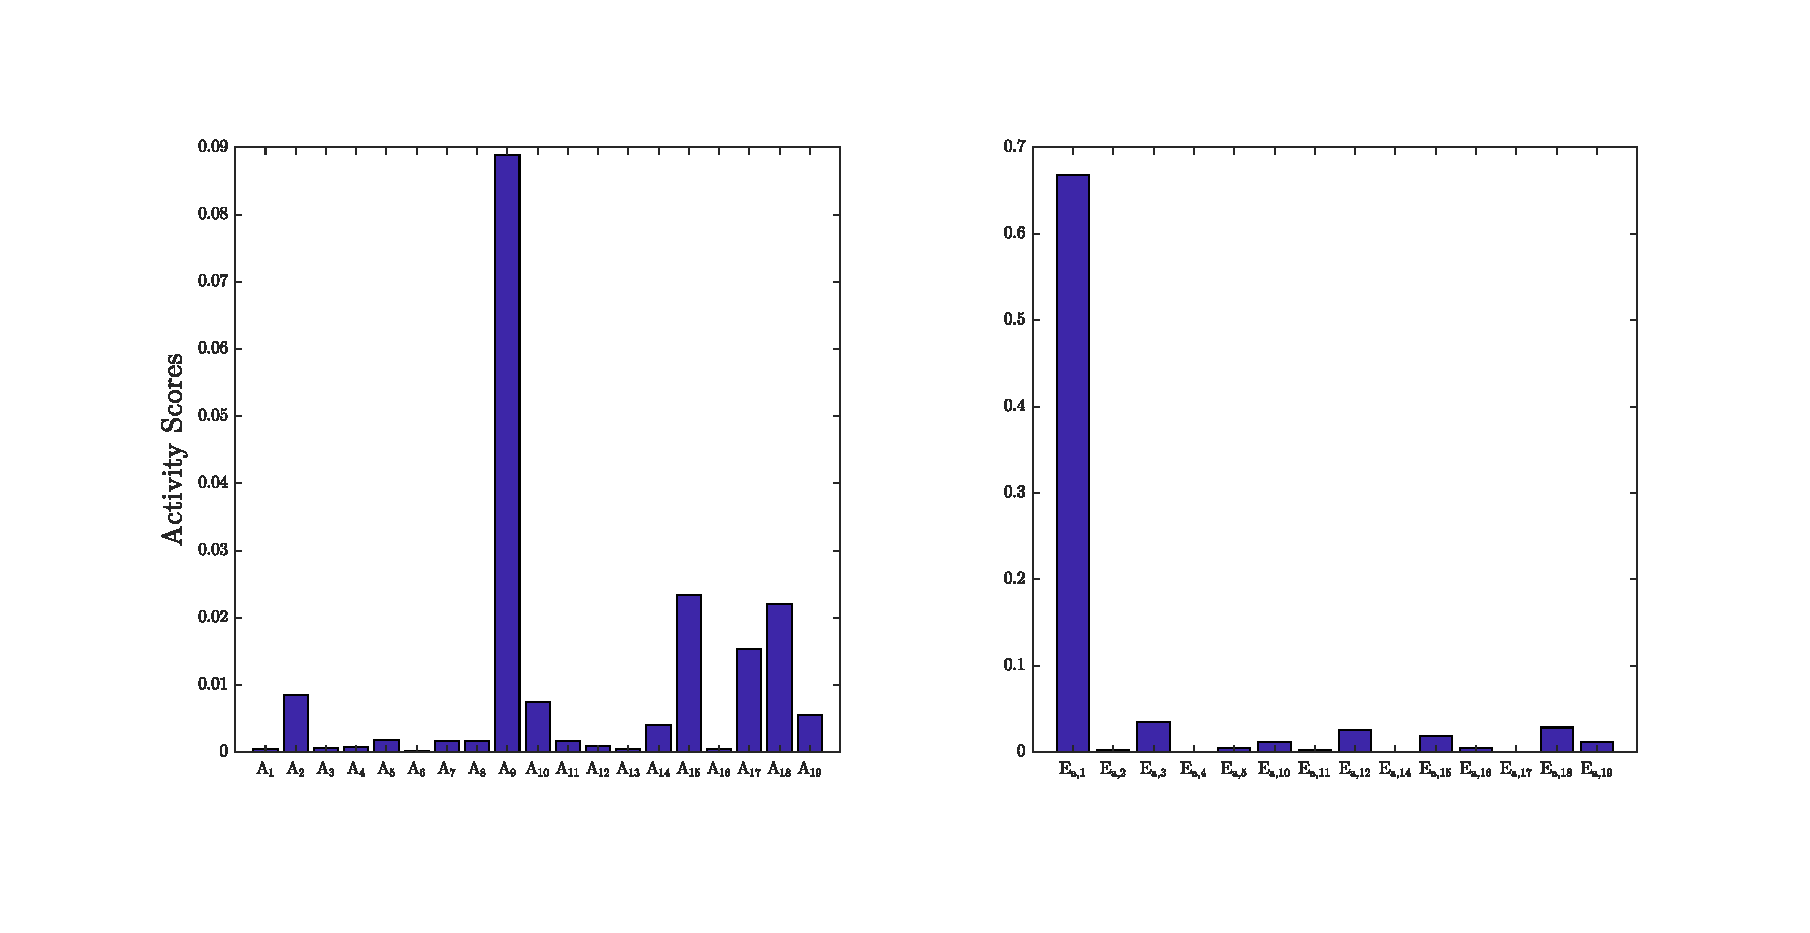
\includegraphics[width=1.1\textwidth]{./Figures/as_33D}
\end{figure}

\end{frame}

\end{document}

















